\documentclass[conference]{IEEEtran}
\usepackage{cite}
\usepackage{amsmath,amssymb,amsfonts}
\usepackage{algorithmic}
\usepackage{graphicx}
\usepackage{textcomp}
\usepackage{xcolor}
\usepackage{booktabs}
\usepackage{array}
\usepackage{url}
\usepackage{subcaption}

% Correct bad hyphenation here
\hyphenation{op-tical net-works semi-con-duc-tor}

\begin{document}

\title{APMS: An Automated Pharmacy System Integrating Prescription OCR, Robotic Dispensing, and AI-Driven Inventory Analytics}

\author{\IEEEauthorblockN{TBD}}

\maketitle

\begin{abstract}
Pharmaceutical dispensing and inventory management represent critical bottlenecks in modern healthcare systems. Manual prescription handling, stock reconciliation, and heuristic reordering often lead to dispensing errors, stockouts, or excessive holding costs. This paper presents the Automated Pharmacy Management System (APMS), an end-to-end integrated hardware-software solution designed to digitize and automate community pharmacy operations from prescription entry to mechanical dispensing and inventory optimization. APMS integrates four core subsystems: (1) an offline, on-premise Prescription OCR pipeline based on a local vision-language model (GLM-OCR) combined with a novel seven-stage sequential fallback search engine that resolves cursive handwriting errors; (2) an adaptive, 3D-printed anthropomorphic robotic hand driven by an MLP neural network that maps ultrasonic palm distances to continuous joint angle trajectories for distance-adaptive grasping; (3) a full-stack software suite (PharmaSys pharmacist dashboard and Roshetety mobile app) featuring real-time WebSocket synchronization; and (4) an AI-driven inventory analytics engine utilizing segmented demand forecasting (LightGBM/Croston's), anomaly detection (ECOD-LOF ensemble), and deep reinforcement learning (Soft Actor-Critic) for optimal replenishment. Empirical evaluations demonstrate that the system achieves a 94.5\% OCR accuracy under controlled lighting, an 85.7\% robotic grasp success rate, and a 59.6\% reduction in total inventory costs compared to traditional min-max policies, proving the viability of low-cost, secure on-premise pharmacy automation.
\end{abstract}

\begin{IEEEkeywords}
Pharmacy Automation, Prescription OCR, Robotic Grasping, Inventory Forecasting, Reinforcement Learning, Soft Actor-Critic.
\end{IEEEkeywords}

\section{Introduction}
The pharmacy industry is currently undergoing a significant digital transformation. Traditional community pharmacies face numerous operational challenges, including manual inventory tracking, paper-based prescription handling, inefficient stock management (leading to either overstocking or stockouts), and a distinct lack of real-time data-driven decision-making. In developing regions, such as Egypt and the broader Middle East, the vast majority of community pharmacies still operate with handwritten paper prescriptions, manual ledger-based inventory systems, and limited technological integration, resulting in significant administrative overhead and dispensing latencies.

Medical errors in pharmaceutical dispensing present a severe threat to patient safety. A primary source of these errors is the misinterpretation of handwritten medical prescriptions. Doctors' handwriting is notoriously difficult to read, and many drug names are visually or phonetically similar (Look-Alike/Sound-Alike or LASA drugs). When pharmacists misread a prescription, they may dispense the wrong medication, wrong dosage, or wrong frequency, with potentially fatal consequences. Automating the extraction and validation of drug names from handwritten prescriptions via Optical Character Recognition (OCR) combined with intelligent search databases represents a crucial safety layer. Furthermore, cloud-based OCR solutions present data privacy concerns under local healthcare regulations, necessitating local, offline processing.

To address these challenges, we propose the \textbf{Automated Pharmacy Management System (APMS)}, an end-to-end framework that bridges digital patient-facing services, intelligent prescription translation, backend pharmacy operations, and on-premise robotic dispensing. The system coordinates patient, pharmacist, and physical hardware actuators in a unified ``Sense-Plan-Act'' cycle. This paper details the hardware and software methodology of the APMS components and presents empirical results demonstrating its performance across OCR accuracy, grasp reliability, and inventory cost reduction.

\section{Related Work}

\textbf{Pharmacy Automation Systems.} Commercial dispensing robots have demonstrated measurable reductions in dispensing errors and labor costs in hospital settings; however, critical evaluations of pharmacy automation~\cite{pharmacy_automation} highlight their high acquisition costs and infrastructure requirements, which place them beyond the reach of small community pharmacies, particularly in developing regions. APMS targets this gap with a low-cost, 3D-printed, on-premise alternative.

\textbf{Handwritten Prescription OCR.} Classical OCR engines such as Tesseract~\cite{tesseract} perform well on printed text but degrade severely on cursive medical handwriting. Deep-learning approaches trained specifically on doctors' cursive handwriting~\cite{cursive_dl} improve recognition but rely on limited drug vocabularies, while commercial cloud services (e.g., Google Cloud Vision) achieve high accuracy at the cost of transmitting patient data to external servers. APMS instead combines a locally hosted vision-language model with a multi-stage lexical/semantic search over a national drug registry, retaining accuracy while keeping data on-premise.

\textbf{Low-Cost Anthropomorphic Hands.} The open-source InMoov project~\cite{inmoov} established the feasibility of 3D-printed, tendon-driven humanoid hands. Mohammadi et al.~\cite{prosthetic} demonstrated a practical soft prosthetic hand with multi-articulating grasp capabilities, and Bulgarelli et al.~\cite{sign_hand} presented a low-cost dexterous anthropomorphic hand for sign-language reproduction. These works validate affordable tendon-driven actuation but target prosthetics and human-robot interaction, whereas APMS adapts this hardware class to autonomous, distance-adaptive dispensing.

\textbf{Demand Forecasting and Replenishment.} Croston's method~\cite{croston} and its accuracy analyses~\cite{syntetos} remain standard for intermittent demand, while gradient-boosting models such as LightGBM~\cite{lightgbm} dominate feature-rich forecasting. For replenishment, deep reinforcement learning has outperformed classical policies in supply-chain benchmarks~\cite{beer_game}; APMS combines segmented forecasting with a Soft Actor-Critic~\cite{sac} reorder agent in one pharmacy-scale engine.

To the best of our knowledge, no prior system integrates offline prescription OCR, low-cost robotic dispensing, and AI-driven inventory analytics into a single end-to-end community pharmacy platform.

\section{System Design and Methodology}

APMS is designed around a unified ``Sense-Plan-Act'' cycle operating across three sequential phases: (A)~Prescription OCR and drug resolution, (B)~Robotic grasping and dispensing, and (C)~Post-order inventory analytics and auditing. A complete order scenario proceeds as follows: the patient initiates the order by photographing a handwritten prescription in the Roshetety mobile app; the on-premise OCR pipeline transcribes and resolves it to verified drug entries; the order appears on the PharmaSys dashboard for pharmacist confirmation; the mobile robot car carrying the anthropomorphic arm then navigates to the target shelf, grasps, and dispenses the medicine; and the logged transaction feeds the post-order analytics engine. The high-level operational execution flow of APMS is illustrated in Fig.~\ref{fig:architecture}.

\begin{figure}[htbp]
\centering
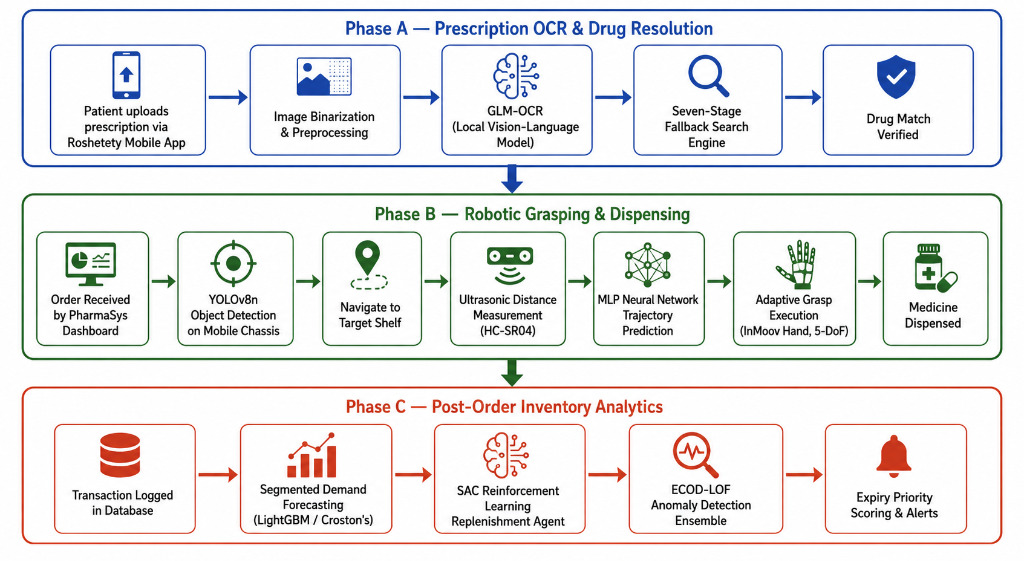
\includegraphics[width=\linewidth]{media/image29.jpg}
\caption{APMS Architectural Execution Flow: Phase~A (Prescription OCR), Phase~B (Robotic Dispensing), and Phase~C (Inventory Analytics).}
\label{fig:architecture}
\end{figure}

\subsection{Phase A: Prescription OCR \& Seven-Stage Fallback Search}
When a patient uploads a prescription via the Roshetety mobile app (Fig.~\ref{fig:ui_screens}a), the order is tracked in real time on the PharmaSys pharmacist dashboard (Fig.~\ref{fig:ui_screens}b) through WebSocket synchronization, and the image is binarized and processed offline by a locally deployed vision-language model (GLM-OCR via Ollama). Since cursive handwriting yields transcription noise, we implement a \textbf{Seven-Stage Sequential Fallback Search Engine} with early-exit confidence thresholds to resolve errors against a unified drug reference database (FDA, EDA, and Vezeeta catalog), diagrammed in Fig.~\ref{fig:search_tree}:
\begin{enumerate}
\item \textbf{Exact Match:} Direct database query. Exit if matched.
\item \textbf{Normalized Match:} Strips spaces, non-alphanumeric characters, and case differences (e.g., ``mil-ga'' $\rightarrow$ ``milga'').
\item \textbf{Smart OCR Fix:} Applies a custom probabilistic visual confusion dictionary modeling optical character errors (e.g., $rn \rightarrow m$, $l \rightarrow 1$, $cl \rightarrow d$) to generate alternative query candidates.
\item \textbf{Elasticsearch Indexing:} Queries an on-premise Elasticsearch node using n-grams and inverted indices.
\item \textbf{Fuzzy Search:} C++ accelerated Jaro-Winkler string distance scoring. It prioritizes prefix similarity. Exits if similarity score $\ge 0.85$.
\item \textbf{Semantic Search:} Computes cosine similarity between Sentence-Transformers~\cite{sentence_bert} dense embeddings of the OCR output and drug categories.
\item \textbf{External Web Crawler Fallback:} REST API requests query the live Vezeeta Egypt directory to catch unindexed local items.
\end{enumerate}

\begin{figure}[htbp]
\centering
\begin{subfigure}[b]{0.24\linewidth}
    \centering
    
\includegraphics[width=\linewidth]{media/image3.jpg}
    \caption{}
\end{subfigure}
\hfill
\begin{subfigure}[b]{0.54\linewidth}
    \centering
    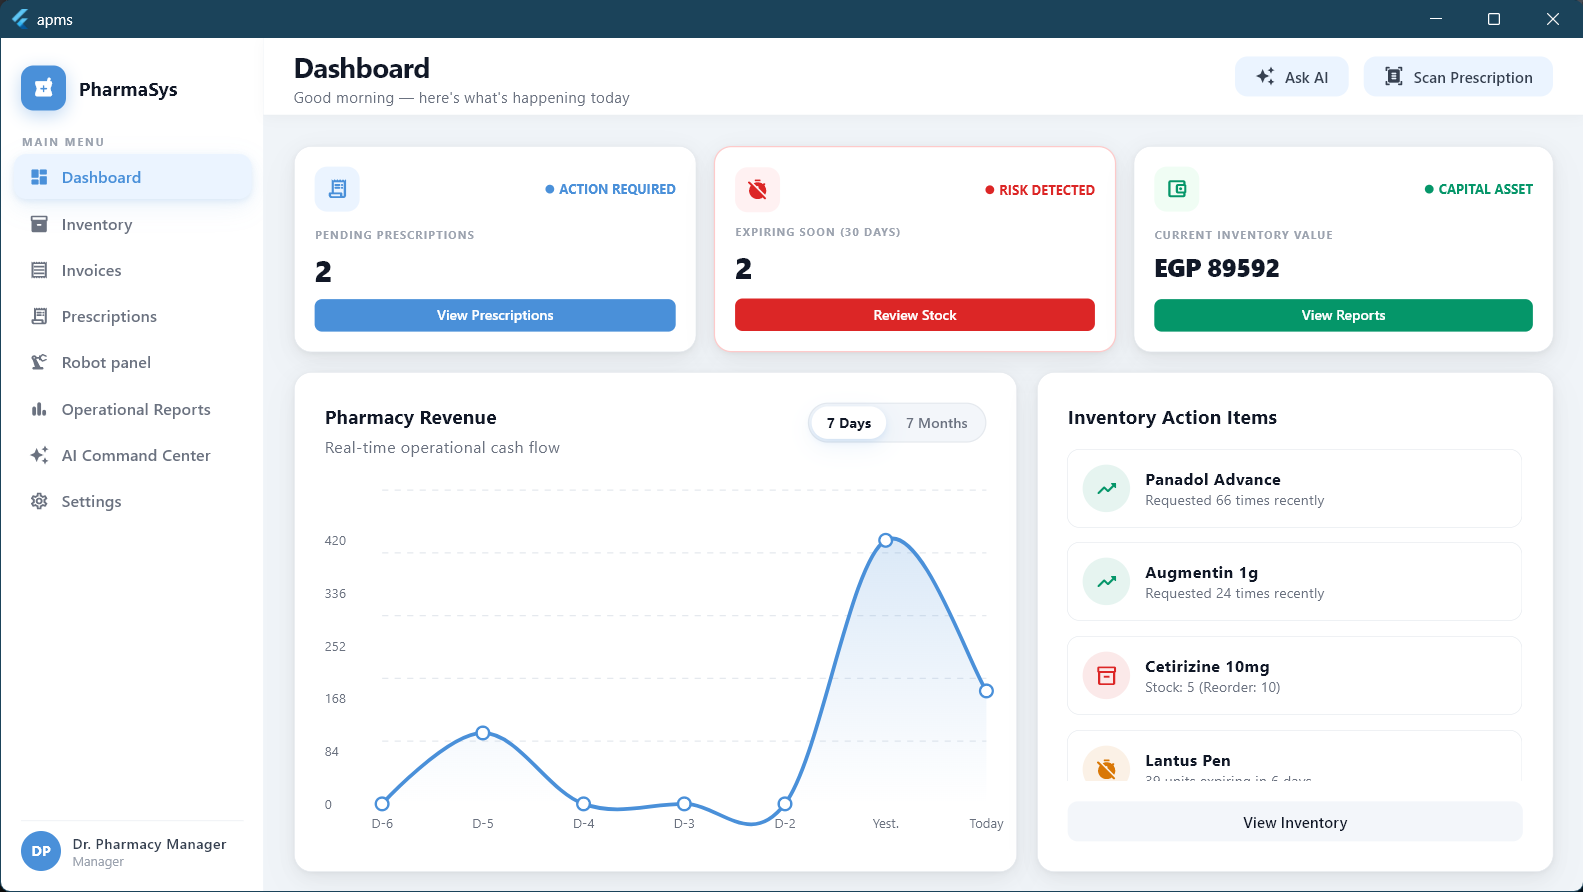
\includegraphics[width=\linewidth]{media/image5.png}
    \caption{}
\end{subfigure}
\caption{APMS user-facing software suite: (a) Roshetety mobile app prescription capture screen (order entry); (b) PharmaSys pharmacist dashboard showing pending prescriptions, expiry alerts, and inventory analytics widgets.}
\label{fig:ui_screens}
\end{figure}

\begin{figure}[htbp]
\centering
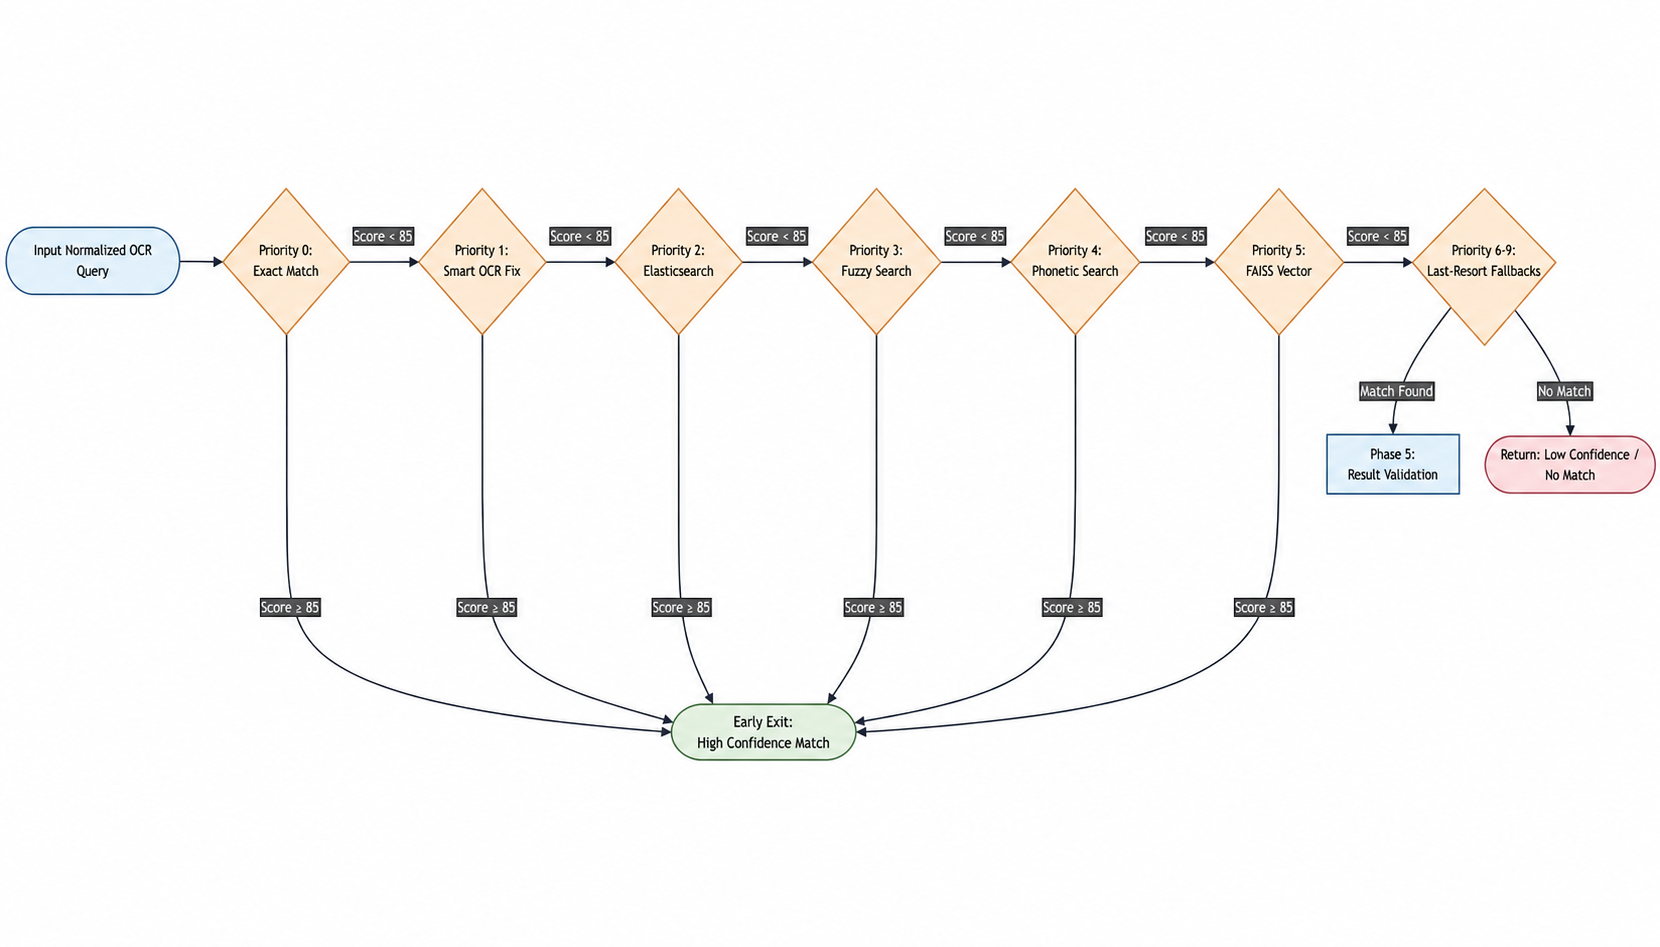
\includegraphics[width=0.62\linewidth]{media/dem_fig.png}
\caption{OCR Seven-Stage Sequential Fallback Search Decision Tree with Early-Exit Confidence Thresholding.}
\label{fig:search_tree}
\end{figure}

The characteristics and prioritization of these search mechanisms are detailed in Table~\ref{tab:search_characteristics}.

\begin{table*}[htbp]
\caption{Characteristics and Priorities of the Fallback Search Stages}
\label{tab:search_characteristics}
\centering
\begin{tabular}{llll}
\toprule
\textbf{Stage} & \textbf{Method} & \textbf{Complexity} & \textbf{Justification for Priority Order} \\
\midrule
0 & Exact Match & $O(1)$ & Instant database lookup, 100\% precision; matches 30--40\% of clear inputs. \\
1 & Normalized Match & $O(1)$ & Resolves spacing/casing variations without executing heavy string metrics. \\
2 & Smart OCR Fix & $O(V \log N)$ & Corrects common handwriting character confusions (e.g., $rn \rightarrow m$) prior to fuzzy scoring. \\
3 & Elasticsearch & $O(\log N)$ & Leverages inverted index and character n-grams for fast approximate retrieval. \\
4 & Fuzzy Search & $O(N \cdot M)$ & Calculates Jaro-Winkler distance; handles arbitrary transcription spelling noise. \\
5 & Semantic Search & $O(D \cdot K)$ & Sentence-Transformers~\cite{sentence_bert} embeddings; resolves severe cursive distortions using semantic context. \\
6 & External Crawler & $O(1)$ & REST query to Egypt drug registry; handles newly registered or unindexed medications. \\
\bottomrule
\end{tabular}
\end{table*}

\subsection{Phase B: Adaptive Grasping Robotic Hand Kinematics}
The physical actuator is an anthropomorphic, 3D-printed, tendon-driven InMoov~\cite{inmoov} hand with 5 active degrees of freedom (DoF), controlled by an ESP32 microcontroller and five MG995 servo motors. The robotic arm is mounted on a mobile wheeled chassis equipped with a YOLOv8n~\cite{yolo} object detection model for visual servo guidance toward the target shelf location.

Each finger is modeled as a serial kinematic chain containing three revolute joints: Metacarpophalangeal (MCP), Proximal Interphalangeal (PIP), and Distal Interphalangeal (DIP) joints. The PIP and DIP joints are coupled mechanically via a shared nylon tendon. Denavit-Hartenberg (D-H) coordinate frames are established at each joint to trace fingertip trajectories relative to the wrist frame, as shown in Fig.~\ref{fig:kinematics}.

\begin{figure}[htbp]
\centering
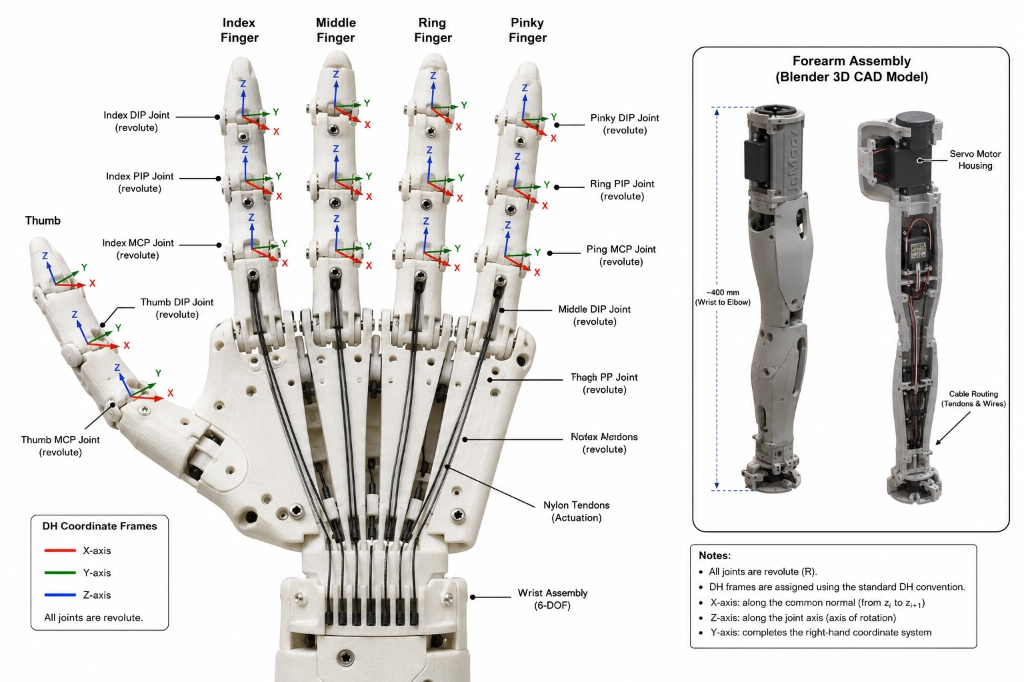
\includegraphics[width=0.75\linewidth]{media/image80.jpg}
\caption{Robotic Kinematics and Blender 3D Design showing DH Coordinate Frames and Blender Forearm Assembly.}
\label{fig:kinematics}
\end{figure}

To map user gesture demonstrations (captured via MediaPipe~\cite{mediapipe} Hand Landmarker during recording) to servo commands, we define the normalized extension ratio $R_i$ for finger $i$:
\begin{equation}
R_i = \frac{\|\mathbf{p}_{\text{tip},i} - \mathbf{p}_{\text{wrist}}\|}{\|\mathbf{p}_{\text{MCP},i} - \mathbf{p}_{\text{wrist}}\|}
\end{equation}
where $\mathbf{p}$ represents the 3D coordinate vectors of the hand landmarks. The target servo command angle $A_i$ (bounded between $A_{\text{open}} = 50^\circ$ and $A_{\text{closed}} = 150^\circ$) is calculated using a linear clamp-and-scale inversion:
\begin{equation}
A_i = \text{clamp}\left( A_{\text{closed}} - \frac{R_i - R_{i,\min}}{R_{i,\max} - R_{i,\min}} \Delta A, \, A_{\text{open}}, \, A_{\text{closed}} \right)
\end{equation}
where $\Delta A = A_{\text{closed}} - A_{\text{open}}$, and $R_{i,\min}$ and $R_{i,\max}$ are the user-specific calibration limits.

To execute autonomous grasping, the hand uses an HC-SR04 ultrasonic sensor mounted on the palm. A Multi-Layer Perceptron (MLP) neural network is trained using backpropagation to map the scalar package distance $d \in [4.0, 9.5]$~cm to a continuous joint trajectory vector of 500 command angles (representing 100 timesteps for the 5 finger servos), enabling distance-adaptive grasp closure.

\subsection{Phase C: AI-Driven Inventory Analytics}\label{sec:analytics}
Following order execution and robotic dispensing, the analytics engine operates as the final phase to optimize capital allocation and audit daily operations.
\subsubsection{Segmented Demand Forecasting}
Products in the inventory are segmented into three classes based on their Average Daily Demand (ADD) computed over the trailing 12~months: \textbf{Fast-Moving} (ADD $\geq$ 1 unit/day), \textbf{Slow-Moving} (0 $<$ ADD $<$ 1 unit/day with $\geq$70\% non-zero months), and \textbf{Intermittent} (all remaining products with sparse, irregular demand). Each class is assigned a specialized forecasting model to capture its distinct demand distribution:
\begin{itemize}
\item \textbf{Fast-Moving:} Modeled using a LightGBM~\cite{lightgbm} regressor trained on engineered features (lag variables of 1, 2, 3, 6, and 12 months, rolling statistics, and cyclical calendar encodings).
\item \textbf{Slow-Moving:} Modeled using Croston's Method~\cite{croston}. It separates the time-series into demand size $z_t$ and interval $p_t$. If demand $y_t > 0$:
\begin{equation}
\hat{z}_t = \hat{z}_{t-1} + \alpha(y_t - \hat{z}_{t-1})
\end{equation}
\begin{equation}
\hat{p}_t = \hat{p}_{t-1} + \alpha(q - \hat{p}_{t-1})
\end{equation}
where $q$ is the elapsed periods since the last sale, and $\alpha \in [0.1, 0.3]$ is the smoothing parameter. If $y_t = 0$, updates are frozen ($\hat{z}_t = \hat{z}_{t-1}$, $\hat{p}_t = \hat{p}_{t-1}$) and $q = q + 1$. The forecast is $\hat{y}_{t+h|t} = \hat{z}_t / \hat{p}_t$.
\item \textbf{Intermittent:} Assigned a trailing 12-month historical average baseline.
\end{itemize}

\subsubsection{Expiry Priority Scoring}
A composite risk score $S$ triggers clearance discounts (up to 40\%) to reduce write-offs:
\begin{equation}
\begin{split}
S = {} & 0.45 S_{\text{expiry}} + 0.25 S_{\text{value}} + 0.15 S_{\text{coverage}} \\
       & + 0.10 S_{\text{demand}} + 0.05 I_{\text{warning}}
\end{split}
\end{equation}
where $S_{\text{expiry}}$ scales inversely with days to expiration, $S_{\text{value}}$ is the financial value, $S_{\text{coverage}}$ is current stock coverage, $S_{\text{demand}}$ is velocity, and $I_{\text{warning}}$ is a binary flag active under 60 days.

\subsubsection{Cashier Shift Anomaly Detection}
To identify recording errors or fraud, we deploy an unsupervised ensemble of Empirical Cumulative Distribution Outlier Detection (ECOD)~\cite{ecod} and Local Outlier Factor (LOF)~\cite{lof}. 
ECOD estimates the ECDF for each dimension $d$ of shift log $x$:
\begin{equation}
\hat{F}_d(x_d) = \frac{1}{N} \sum_{i=1}^{N} I(x_{i,d} \le x_d)
\end{equation}
and computes an anomaly score based on tail probabilities:
\begin{equation}
O_{\text{ECOD}}(x) = \sum_{d=1}^{D} \max\left(-\log \hat{F}_d(x_d), -\log(1 - \hat{F}_d(x_d))\right)
\end{equation}
LOF measures the local density deviation of $x$ relative to its $k$-nearest neighbors:
\begin{equation}
\text{LOF}_k(p) = \frac{\sum_{o \in N_k(p)} \frac{\text{lrd}_k(o)}{\text{lrd}_k(p)}}{|N_k(p)|}
\end{equation}
where $\text{lrd}$ is the local reachability density. A consensus flag is raised only if both models mark the shift as anomalous.

\subsubsection{Reinforcement Learning Replenishment}
Stock reordering is formulated as a Markov Decision Process (MDP) with a 5-dimensional state space $x_t = [I_t, D_t, V_t, C_t, R_t]^T$, representing inventory level, days since last order, rolling demand, coverage, and reorder ratio. A continuous-action Soft Actor-Critic (SAC)~\cite{sac} reinforcement learning agent is trained in a simulator calibrated on historical transaction data to maximize cumulative reward:
\begin{equation}
\begin{split}
R = {} & \text{Revenue} - \text{Ordering Cost} \\
       & - \text{Holding Cost} - \text{Stockout Penalty}
\end{split}
\end{equation}

\section{Experimental Results and Discussion}
The experimental results are presented in the same sequential order as the methodology phases: Phase~A (OCR), Phase~B (Robotic Grasping), and Phase~C (Inventory Analytics).

\subsection{Phase A Results: OCR Performance and Environmental Lighting}
The local GLM-OCR model was evaluated under three lighting conditions across 200 package samples. Under optimal bright lighting (250 lm), the OCR achieved a 94.5\% overall recognition rate. Accuracy dropped to 88.5\% under moderate light (100 lm) and 71.0\% under dim light (15 lm), showing high dependency on ambient contrast. Incorporating an internal LED strip inside the camera housing resolved the dim-light drop-off.

Furthermore, we compared the APMS OCR pipeline against standard Tesseract v5.3~\cite{tesseract} and commercial Google Cloud Vision API on a validation set of 500 handwritten prescriptions. The results in Table~\ref{tab:ocr_comparison} show that APMS local GLM-OCR balances high accuracy (8.5\% Character Error Rate) with absolute on-premise data privacy and offline support. Latency measures the end-to-end time from image submission to final medicine name resolution at the server level. The \emph{Privacy} column indicates whether patient prescription data leaves the pharmacy premises (``Local'' = fully on-premise; ``Cloud'' = transmitted to external servers).

\begin{table}[htbp]
\caption{Comparison of OCR Engines on Handwritten Prescriptions}
\label{tab:ocr_comparison}
\centering
\setlength{\tabcolsep}{4.5pt}
\begin{tabular}{lcccc}
\toprule
\textbf{OCR Engine} & \textbf{CER (\%)} & \textbf{WER (\%)} & \textbf{Latency (s)} & \textbf{Privacy} \\
\midrule
Tesseract v5.3 & 38.4\% & 62.3\% & 0.4 & Local \\
Google Cloud Vision & 7.2\% & 11.5\% & 2.5 & Cloud \\
\textbf{APMS GLM-OCR} & \textbf{8.5\%} & \textbf{14.2\%} & \textbf{1.8} & \textbf{Local} \\
\bottomrule
\end{tabular}
\end{table}

\subsection{Phase B Results: Robotic Grasping Success Rates}
The physical performance of the InMoov hand was evaluated across 300 experimental trials (50 trials per distance step) on standard medicine boxes. A grasp was classified as successful if the object was lifted and retained for 6 seconds. The success rate at each distance is computed as the ratio of successful grasps to the 50 trials conducted at that distance (e.g., 46/50 = 92.0\% at 5.0~cm). The results are summarized in Table~\ref{tab:grasp_success}.

\begin{table}[htbp]
\caption{Robotic Grasping Success Rate by Target Distance}
\label{tab:grasp_success}
\centering
\begin{tabular}{cc>{\raggedright\arraybackslash}p{3.5cm}}
\toprule
\textbf{Distance (cm)} & \textbf{Success Rate (\%)} & \textbf{Notes} \\
\midrule
4.0 & 88.0\% (44/50) & Occasional over-squeeze at min.\ range \\
5.0 & 92.0\% (46/50) & Optimal; matches training centroid \\
6.0 & 90.0\% (45/50) & Consistent, reliable grasping \\
7.0 & 86.0\% (43/50) & Minor tendon slippage observed \\
8.0 & 82.0\% (41/50) & Interpolation boundary \\
9.0 & 76.0\% (38/50) & Reduced grip near max.\ limit \\
\midrule
\textbf{Overall} & \textbf{85.7\% (257/300)} & \textbf{Avg.\ across operational space} \\
\bottomrule
\end{tabular}
\end{table}

\subsubsection{Object Detection for Mobile Chassis Navigation}
To deploy visual guidance on the mobile wheeled chassis that carries the robotic arm to the target shelf, we compared the standard YOLOv8 Nano (YOLOv8n)~\cite{yolo} against a parameter-pruned YOLO26n. Although YOLO26n utilizes 36\% fewer GFLOPs, YOLOv8n converged 2.3$\times$ faster (mAP@50 $>$ 0.9 by epoch 3 vs. epoch 7) and demonstrated a 12\% lower inference latency (2.9ms vs. 3.3ms), making it highly suitable for visual servo loop control (Table~\ref{tab:yolo_comparison}).

\begin{table}[htbp]
\caption{YOLOv8n vs. YOLO26n Performance Comparison}
\label{tab:yolo_comparison}
\centering
\begin{tabular}{lcc}
\toprule
\textbf{Metric} & \textbf{YOLOv8n} & \textbf{YOLO26n} \\
\midrule
Trainable Parameters & 3,006,233 & 2,375,421 \\
GFLOPs & 8.1 & 5.2 \\
Peak mAP@50 & 0.9950 & 0.9950 \\
Peak mAP@50-95 & 0.9740 & 0.9800 \\
Inference Latency & 2.9ms & 3.3ms \\
\bottomrule
\end{tabular}
\end{table}

\subsubsection{3D Printing Infill Density Characterization}
Tensile specimens were characterization-tested to determine the optimal balance between physical weight and structural load durability. The selection criteria were: (1)~total part mass must remain below the MG995 servo rated torque limit of 12~kg$\cdot$cm, (2)~print time must be minimized for rapid prototyping iterations, and (3)~the part must withstand repeated grasp forces without deformation. Grid infill configurations at 25\% density exhibited the lowest mass (12.5g for grid vs. 14.8g for gyroid) and minimal print times (Fig.~\ref{fig:infill_char}). Therefore, a 25\%--30\% grid infill was selected for fingers and structural links, reducing arm weight by 40\% and preventing MG995 motor overload under rated torque (12~kg$\cdot$cm).

\begin{figure}[htbp]
\centering
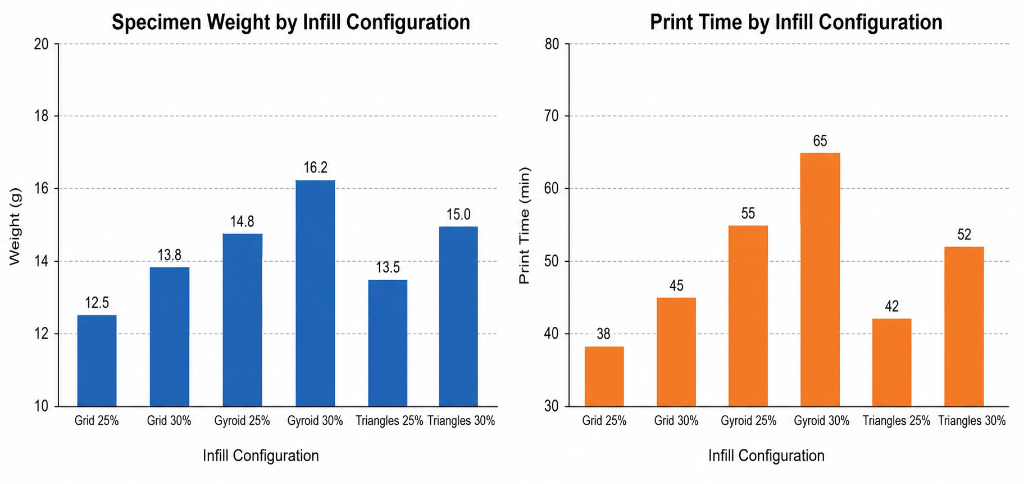
\includegraphics[width=0.78\linewidth]{media/image15.jpg}
\caption{Effect of infill pattern and density on specimen weight and print time.}
\label{fig:infill_char}
\end{figure}

\subsection{Phase C Results: Demand Forecasting and Inventory Optimization}
As part of the post-order analytics phase (Phase~C), the forecasting models were trained on 60 months of historical transactions. Segmenting products by demand profile (as described in Section~\ref{sec:analytics}) yielded significant performance increases over global models, as shown in Table~\ref{tab:forecasting_results}.

\begin{table}[htbp]
\caption{Demand Forecasting Results by Segment (Phase~C Analytics)}
\label{tab:forecasting_results}
\centering
\begin{tabular}{llccc}
\toprule
\textbf{Segment} & \textbf{Model} & \textbf{n} & \textbf{$R^2$ (\%)} & \textbf{RMSE} \\
\midrule
\mbox{Fast-Moving} & LightGBM~\cite{lightgbm} & 736 & 19.52\% & 52.69 \\
\mbox{Slow-Moving} & Croston's~\cite{croston} & 1,329 & 2.23\% & 12.53 \\
\mbox{Intermittent} & Hist. Average & 6,518 & Baseline & 17.04 \\
\bottomrule
\end{tabular}
\end{table}

For replenishment, the SAC~\cite{sac} agent was compared against standard rule-based heuristics---Fixed Reorder Point~\cite{reorder_policies} and Min-Max Inventory~\cite{reorder_policies}---inside the simulation environment. Over 200,000 steps, the SAC policy converged, achieving a \textbf{59.6\% cost reduction} over both baseline policies (Table~\ref{tab:reorder_results}).

\begin{table}[htbp]
\caption{Reorder Policy Performance Comparison}
\label{tab:reorder_results}
\centering
\begin{tabular}{lcc}
\toprule
\textbf{Replenishment Method} & \textbf{Mean Reward} & \textbf{Cost Reduction (\%)} \\
\midrule
Fixed Reorder Point~\cite{reorder_policies} & 361.33 & -- \\
Min-Max Inventory~\cite{reorder_policies} & 363.35 & -- \\
\textbf{SAC Agent (200k steps)} & \textbf{579.84} & \textbf{+59.6\%} \\
\bottomrule
\end{tabular}
\end{table}

\subsection{Phase C Results: Shift Anomaly Auditing Consensus}
The ECOD~\cite{ecod}--LOF~\cite{lof} anomaly ensemble processed 1,000 daily cashier shift records. The models achieved a strong statistical consensus with a \textbf{97.4\% agreement rate} (974 out of 1,000 shifts flagged identically). The ensemble flagged 33 shifts (3.3\%) as high-risk discrepancies, illustrating a robust unsupervised audit tool.

\section{Conclusions and Future Work}
This paper presented the methodology and experimental results of the APMS community pharmacy automation system. The offline GLM-OCR pipeline achieves high transcription accuracy (8.5\% CER) while securing patient data sovereignty. The MLP-driven tendon InMoov hand demonstrates robust adaptive grasping (85.7\% success), and the SAC replenishment agent cuts inventory logistics costs by 59.6\%. Future work will focus on integrating TensorRT optimizations to reduce local VLM latency below 300 milliseconds.

\begin{thebibliography}{99}
\bibitem{inmoov} G. Langevin, ``InMoov: The first life-size humanoid robot you can 3D print and animate,'' Available: \url{https://inmoov.fr/project}.
\bibitem{prosthetic} A. Mohammadi, J. Lavranos, P. Choong, and D. Oetomo, ``A practical 3D-printed soft robotic prosthetic hand with multi-articulating capabilities,'' \emph{PLOS ONE}, vol. 15, no. 5, p. e0232766, 2020.
\bibitem{sign_hand} A. Bulgarelli et al., ``A low-cost open source 3D-printable dexterous anthropomorphic robotic hand with a parallel spherical joint wrist for sign languages reproduction,'' \emph{Int. J. Adv. Robotic Systems}, vol. 13, no. 3, 2016.
\bibitem{mediapipe} C. Lugaresi et al., ``MediaPipe: A framework for building perception pipelines,'' \emph{arXiv preprint arXiv:1906.08172}, 2019.
\bibitem{croston} J. D. Croston, ``Forecasting and stock control for intermittent demands,'' \emph{J. Oper. Res. Soc.}, vol. 23, no. 3, pp. 289--301, 1972.
\bibitem{lightgbm} G. Ke et al., ``LightGBM: A highly efficient gradient boosting decision tree,'' in \emph{Advances in Neural Information Processing Systems}, vol. 30, 2017.
\bibitem{sac} T. Haarnoja, A. Zhou, P. Abbeel, and S. Levine, ``Soft actor-critic: Off-policy maximum entropy deep reinforcement learning with a stochastic actor,'' in \emph{Proc. Int. Conf. Machine Learning (ICML)}, 2018.
\bibitem{ecod} Z. Li et al., ``ECOD: Unsupervised outlier detection using empirical cumulative distribution functions,'' \emph{arXiv preprint arXiv:2201.00382}, 2022.
\bibitem{lof} M. M. Breunig et al., ``LOF: Identifying density-based local outliers,'' in \emph{Proc. ACM SIGMOD Int. Conf. Management of Data}, 2000.
\bibitem{yolo} M. Talib, A. H. Y. Al-Noori, and J. Suad, ``YOLOv8-CAB: Improved YOLOv8 for real-time object detection,'' \emph{Karbala Int. J. Modern Sci.}, vol. 10, no. 1, 2024.
\bibitem{sentence_bert} N. Reimers and I. Gurevych, ``Sentence-BERT: Sentence embeddings using Siamese BERT-networks,'' in \emph{Proc. EMNLP}, 2019.
\bibitem{reorder_policies} E. A. Silver, D. F. Pyke, and D. J. Thomas, \emph{Inventory and Production Management in Supply Chains}, 4th ed. Boca Raton, FL, USA: CRC Press, 2017.
\bibitem{pharmacy_automation} A. M. Boyd and B. W. Chaffee, ``Critical evaluation of pharmacy automation and robotic systems: A call to action,'' \emph{Hospital Pharmacy}, vol. 54, no. 1, pp. 4--11, 2019.
\bibitem{tesseract} R. Smith, ``An overview of the Tesseract OCR engine,'' in \emph{Proc. Int. Conf. Document Analysis and Recognition (ICDAR)}, 2007, pp. 629--633.
\bibitem{cursive_dl} L. J. Fajardo et al., ``Doctor's cursive handwriting recognition system using deep learning,'' in \emph{Proc. IEEE HNICEM}, 2019.
\bibitem{syntetos} A. A. Syntetos and J. E. Boylan, ``The accuracy of intermittent demand estimates,'' \emph{Int. J. Forecasting}, vol. 21, no. 2, pp. 303--314, 2005.
\bibitem{beer_game} A. Oroojlooyjadid, M. Nazari, L. V. Snyder, and M. Tak\'a\v{c}, ``A deep Q-network for the beer game: Deep reinforcement learning for inventory optimization,'' \emph{Manuf. Serv. Oper. Manag.}, vol. 24, no. 1, pp. 285--304, 2022.
\end{thebibliography}

\end{document}
